\documentclass[border=10pt]{standalone}
\usepackage{tikz}
\usepackage{pgfplots}
\pgfplotsset{compat=1.18}

\begin{document}
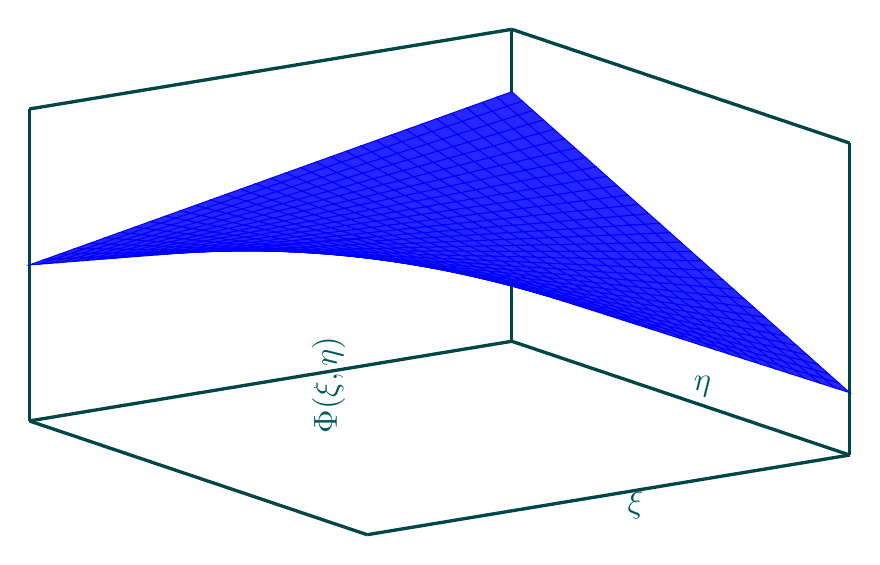
\begin{tikzpicture}
    \begin{axis}[
        width=12cm,
        height=8cm,
        view={-35}{24},
        axis lines=box,
        xmin=0, xmax=1,
        ymin=0, ymax=1,
        zmin=0, zmax=1,
        xtick=\empty,
        ytick=\empty,
        ztick=\empty,
        clip=false,
        axis line style={teal!55!black, very thick},
        label style={teal!70!black},
        enlargelimits=false,
    ]
        % Add labels to the axes
        \node[teal!70!black, font=\large] at (axis cs:0.50,-0.08,0) {$\xi$};
        \node[teal!70!black, font=\large] at (axis cs:1.08,0.55,0) {$\eta$};
        \node[teal!70!black, font=\large, rotate=90] at (axis cs:-0.08,0,0.50) {$\Phi(\xi,\eta)$};

        % Fill the surface with a grid pattern
        \addplot3[
            surf,
            shader=faceted,
            faceted color=blue,
            draw=blue,
            line width=0.35pt,
            samples=33,
            samples y=33,
            domain=0:1,
            y domain=0:1,
            colormap={solidblue}{color=(blue!85) color=(blue!85)},
            point meta=0,
        ] {0.95 - 0.75*x - 0.45*y + 1.05*x*y};
    \end{axis}
\end{tikzpicture}
\end{document}
